\documentclass{beamer}
\usepackage[italian]{babel}
\usepackage[autostyle, english = american]{csquotes}
\usepackage{graphicx}
\usepackage{parskip}
\usepackage{subcaption}
\usetheme{Boadilla}
\graphicspath{ {./} }
\begin{document}
\title{Esercitazione 9}
\subtitle{Remote Procedure Call (RPC) - II}
\author{Corradini, De Luca, di Nuzzo, Frick, Ragazzini}
\institute{unibo}
\date{2019}
\setbeamercovered{transparent}
\begin{frame}
\titlepage
\end{frame}
\begin{frame}
    \frametitle{XDR}

    Il file \texttt{fattore.x} definisce le strutture:
    \begin{itemize}
        \item \texttt{Input}: contiene i campi \texttt{nome} e \texttt{operazione} che corrispondono rispettivamente al nome del candidato su cui operare e all'operazione da effettuare;
        \item \texttt{Giudice}: contiene solo il campo \texttt{nome};
        \item \texttt{Output}: contiene il campo \texttt{giudici} che funge da indice per la struttura dati che mantiene lo stato del server.
    \end{itemize}
    Il file definisce inoltre le procedure remote \texttt{esprimi\_voto()} e \texttt{classifica\_giudici()}.

\end{frame}
\begin{frame}
    \frametitle{Cliente}

    Il cliente richiede ciclicamente il tipo di operazione da eseguire e lo salva nella stringa \texttt{op}, dimensionata opportunamente in modo da contenere il carattere:\begin{itemize}
        \item \texttt{'1'} per invocare \texttt{classifica\_giudici\_1()} che calcola i voti totali ottenuti dai candidati facenti riferimento a ciascun giudice, ordina i giudici in base ai punteggi totali con un algoritmo di \textit{selection sort} e restituisce la classifica ordinata;
        \item \texttt{'2'} per invocare \texttt{esprimi\_voto\_1()} passandogli come argomento la stringa \texttt{"aggiunta"} per aggiungere un voto a un candidato;
        \item \texttt{'3'} per invocare \texttt{esprimi\_voto\_1()} passandogli come argomento la stringa \texttt{"sottrazione"} per sottrarre un voto a un candidato;
    \end{itemize}
    e il terminatore di stringa.

    Gli unici comandi accettati sono \texttt{'1'}, \texttt{'2'}, \texttt{'3'} e \textit{EOF}.

\end{frame}
\begin{frame}
    \frametitle{Servitore}
Il servitore implementa le funzioni \texttt{esprimi\_voto\_1()} e \texttt{classifica\_giudici\_1()}.
\begin{itemize}
    \item \texttt{esprimi\_voto\_1()} prende come argomenti il nome di un candidato e una stringa, che può essere \texttt{"aggiunta"} o \texttt{"sottrazione"}. La procedura cerca il nome del candidato in una opportuna struttura dati, restituendo un errore (che viene gestito dal client) nel caso il candidato non esista. Se il candidato esiste, incrementa o decrementa il numero dei suoi voti, controllando che non scendano sotto 0, e restituisce il nuovo punteggio del candidato.
    \item \texttt{classifica\_giudici\_1()} cicla sulla struttura dati aggiornando i voti totali corrispondenti a ogni candidato (politica di aggiornamento \textit{pigro}: i voti totali vengono conteggiati solo quando è richiesta la classifica), poi restituisce la lista di giudici ordinati in base ai voti.
\end{itemize}

\end{frame}
\begin{frame}
    \frametitle{Profilazione dell'esecuzione in locale}
    \begin{figure}[ht]
        \centering
        
        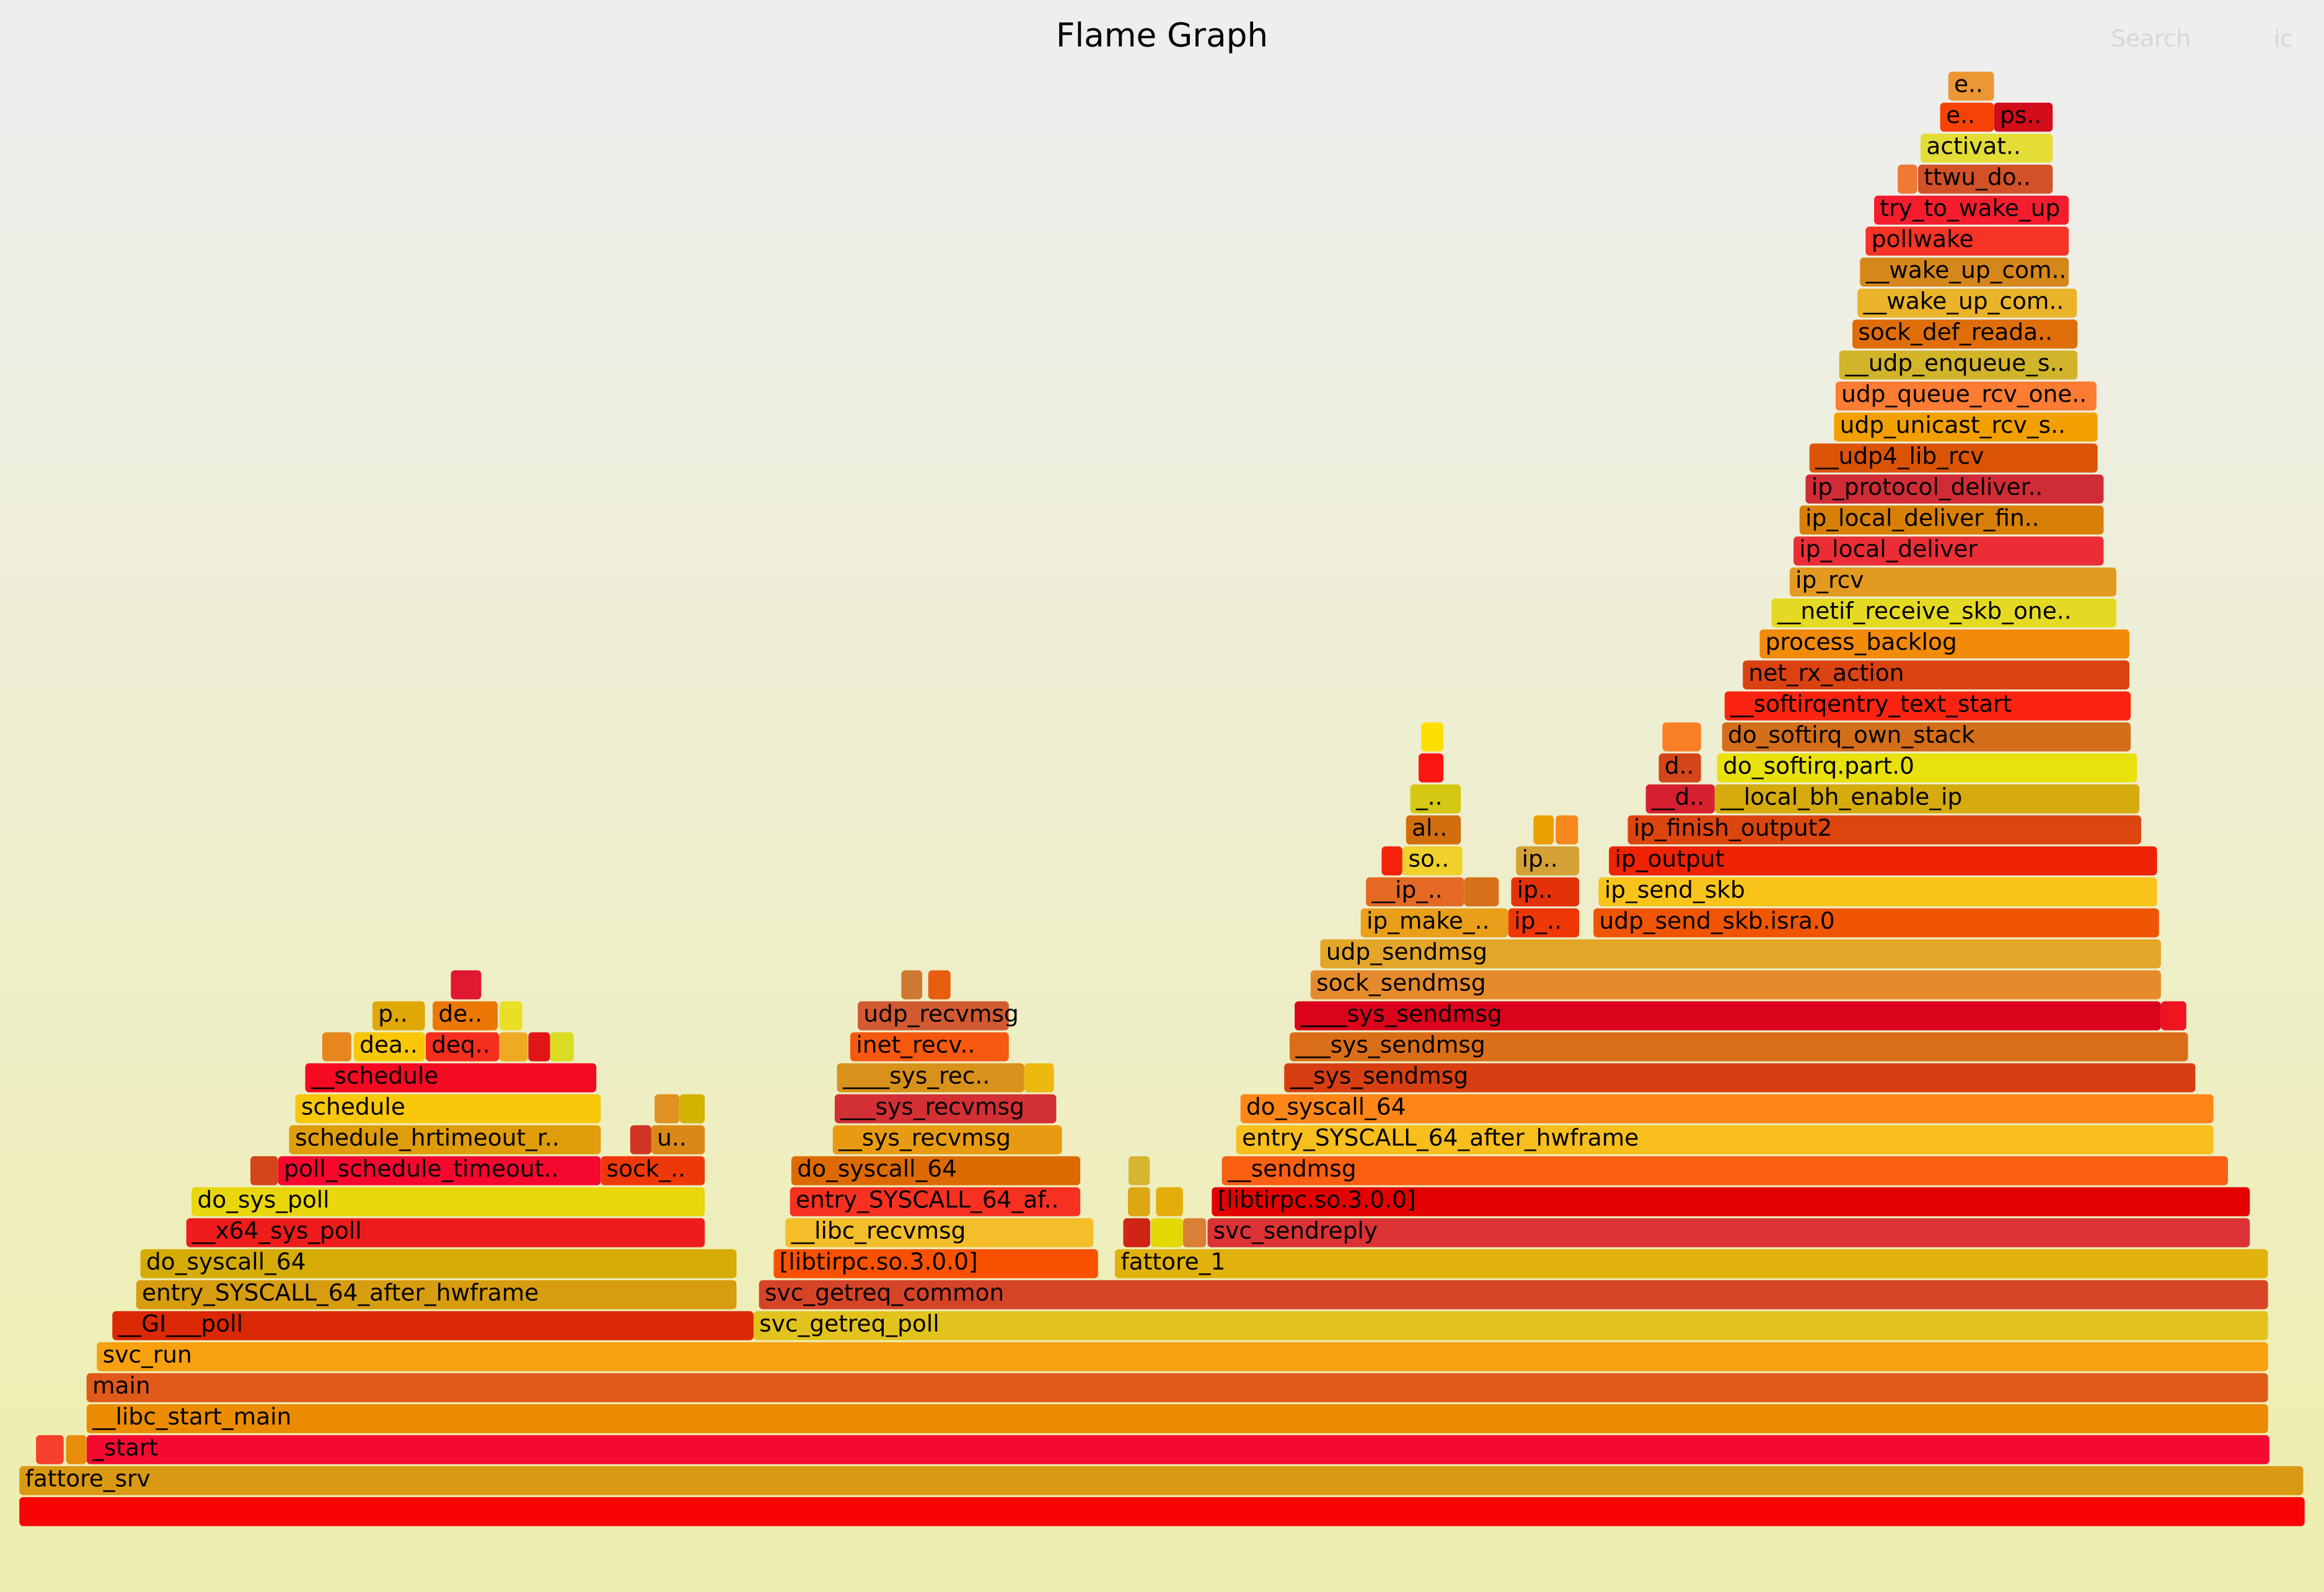
\includegraphics[width = 0.75\textwidth]{fattore.png}
        
        \caption{Grafico a fiamma dell'esecuzione di circa 84000 richieste in locale, attribuendo voti a candidati diversi e chiamando la funzione di ordinamento ogni 5 votazioni.}
        \label{fig:local}
    \end{figure}    

\end{frame}
\begin{frame}
    \frametitle{Conclusioni}
    \begin{itemize}
        \item I tempi di esecuzione delle due procedure remote sono pressoché uguali;
        \item L'\textit{overhead} introdotto da RPC è di svariate volte maggiore del tempo di esecuzione delle procedure remote.
    \end{itemize}
\end{frame}
\end{document}
